\paragraph{Загрузка модели в промежуточный проект}

Приложения, разработанные на основе фреймворка Unity не имею встроенной возможности
к загрузке произвольных трехмерных моделей непосредственно с дискового накопителя.
Модели в Unity могут загружаться одним из следующих способов:

\begin{itemize}
    \item {
        Модель должна быть непосредственно загружена в проект
        разрабатываемого приложения до его компиляции.
        После этого она может загружаться в запущенном приложении
        за счет внутреннего механизма сериализации данных.
        Данный подход очевидно является неприменимым в нашем случае,
        так как он приведет к встраиванию информационной модели в приложение. 
    }
    \item {
        Загрузка модели может осуществляться за счет
        специализированного отдельно разработанного модуля,
        включенного в клиентскую часть прототипа.
        Такое решение будет слишком трудоемко для разработки в рамках прототипа. 
    }
    \item {
        Загрузка моделей может производиться с помощью встроенной в фреймворк
        системы динамической загрузки стороннего контента.
        Загружаемый контент должен предварительно упаковывать
        в специальные файлы, создание которых возможно только
        с помощью редактора Unity.
    }
\end{itemize}

Таким образом, вторым этапом обработки модели является подготовка модели к упаковке
через ее добавление в промежуточный проект редактора Unity.
К счастью, программный интерфейс редактора Unity полностью покрывает
все наши нужды, тем самым весь дальнейший процесс поддается полной автоматизации.

Для автоматического импортирования моделей в промежуточный проект
необходимо создать скрипт, который можно запускать из командной строки
без участия пользователя.\cite{DocUnity}
Общий алгоритм импорта моделей показан на рисунке~\ref{figure:SImportModels}.

\begin{figure}[ht]
    \centering
    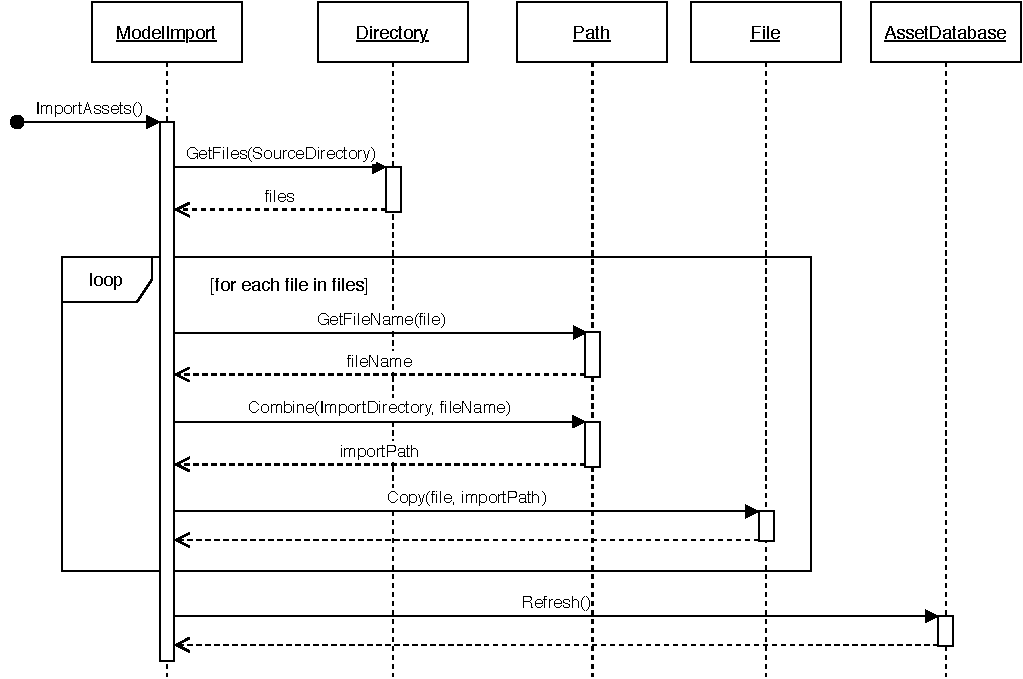
\includegraphics[width=1.0\textwidth]{images/UML-SImportModels.pdf}
    \caption{Импорт моделей.}
    \label{figure:SImportModels}
\end{figure}

Для импорта новых ресурсов в проект Unity необходимо скопировать
файлы в директорию проекта (\emph{<путь к проекту>/Assets})
и вызвать метод обновления базы данных ресурсов Unity (\emph{AssetDatabase}),
что приведет к импорту всех новых или измененных ресурсов,
а также отчистке базы данных от уже несуществующих.%
\cite{DocUnity}

На стадии импорта моделей можно также проводить извлечение
сохранившейся в модели атрибутивной информации.
Для этого нам потребуется создать специальный обработчик моделей
(рисунок~\ref{figure:CPostprocessor}). 

\begin{figure}[ht]
    \centering
    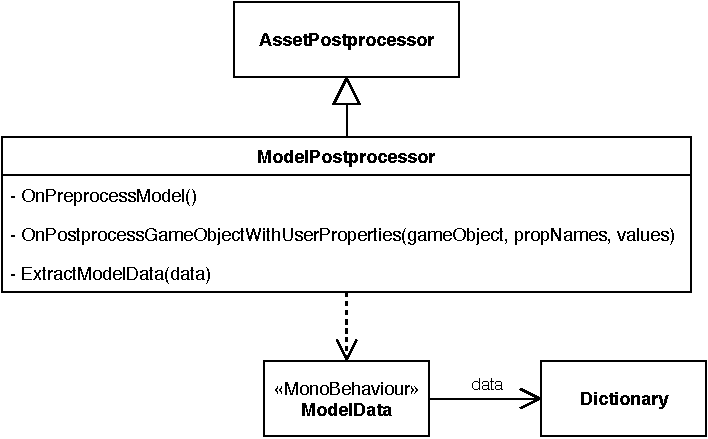
\includegraphics[width=0.6\textwidth]{images/UML-CPostprocessor.pdf}
    \caption{Постобработчик моделей.}
    \label{figure:CPostprocessor}
\end{figure}

Для обработки ресурсов на различных стадиях импорта в проект Unity,
например до начала импорта или после его завершения при определенных условиях,
в проекте реализуется наследник класса \emph{AssetPostprocessor}.
Для задания необходимого поведения при обработке ресурсов
в классе-наследнике реализуются набор специальных методов:
\emph{OnPreprocessModel} -- метод, позволяющий задать настройки импорта до его начала
(в нашем случае необходимо задать генерацию данных для внутренней
системы Unity по обработке физических коллизий);
\emph{OnPostprocessGameObjectWithUserProperties} -- метод, позволяющий
обработать импортированный ресурс, если у него были найдены
``определенные пользователем свойства'', что в нашем случае
является атрибутивной информацией модели.%
\cite{DocUnity}
Извлеченная атрибутивная информация сохраняется в вспомогательно объекте
(\emph{ModelData}) в формате ключ-значение.
Сам процесс извлечения атрибутивной информации показан
на рисунке~\ref{figure:SPostprocessor}.

\begin{figure}[ht]
    \centering
    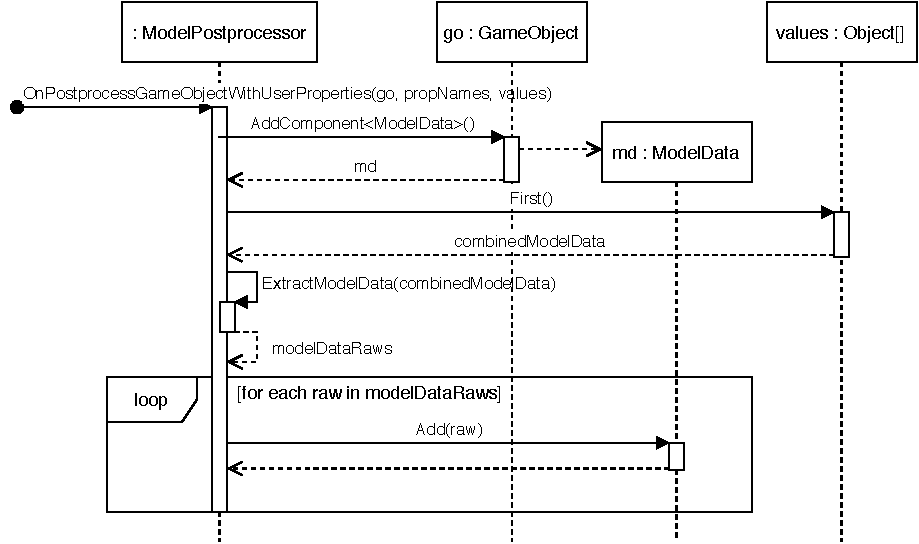
\includegraphics[width=1.0\textwidth]{images/UML-SPostprocessor.pdf}
    \caption{Извлечение атрибутивной информации модели.}
    \label{figure:SPostprocessor}
\end{figure}

Извлекаемая атрибутивная хранится в первом элементе
входного массива \emph{values} в текстовом виде.%
\cite{DocUnity}
Для извлечения информации из полученной строки используется метод
\emph{ExtractModelData}, возвращающий извлеченную атрибутивную информацию
в виде массива ключ-значение.
После чего извлеченная информация сохраняется в компоненте \emph{ModelData},
добавленном к обрабатываемому объекту.
